\section{Creative destruction: an economic implications bridge}
\label{app:economics}

\subsection{From value anchors to adjustment channels}
Creative destruction links technological opportunity to displacement, rent allocation,
and institutional adaptation \citep{schumpeter1942capitalism,aghion1992model,mokyr2002gifts,nobel2025}.
The six survey anchors do not observe economic decisions, but they measure preferences
that can enter the framing of those decisions. We organize the connection without
collapsing the anchors into a fitted welfare index:

\begin{table}[!htbp]
\centering
\caption{Theory-indexed interpretation of the measured anchors.}
\label{tab:economic-channels}
\small
\begin{tabular}{p{0.20\linewidth}p{0.28\linewidth}p{0.40\linewidth}}
\toprule
\rowcolor{tablehead}
Creative-destruction margin & Observed anchors & Potential implication when used by an AI adviser \\
\midrule
Opportunity and participation & science, agency & expectations about innovation gains and who can act on them \\
Distribution and adjustment & income equality/incentives, government/individual responsibility & framing of rents, compensation, retraining, and safety-net responsibility \\
Coordination and legitimacy & trust, immigration impact & expectations about cooperation, mobility, and political acceptance of transition \\
\bottomrule
\end{tabular}
\end{table}

The empirically strongest GPT-5.6 improvements occur on the two anchors in the
distribution-and-adjustment row. At the same time, cross-country geometry does not show
a conclusive improvement. The resulting implication is asymmetric: the update more
accurately represents selected preferences about distribution and responsibility, while
the relational conditions that shape collective adjustment remain statistically
unresolved.

\subsection{An empirical implications index}
For country $c$, model $m$, and margin $g$, let
$L_{mcg}=|J_g|^{-1}\sum_{j\in J_g}\mathrm{TVD}_{mcj}^2$, where each $J_g$ contains the
two anchors in Table~\ref{tab:economic-channels}. Squaring makes larger distributional
mismatches more influential without imposing a sign on the underlying value scale. The
three margin contrasts use the same country bootstrap and paired sign flips as the main
analysis, with Holm correction across margins. For any declared weight vector
$w\in\Delta^2$, the overall implications index is $L_{mc}(w)=\sum_gw_gL_{mcg}$. We
evaluate every 0.02 grid point on the simplex rather than select weights after seeing the
result.

Figure~\ref{fig:economic-story} reports the margin estimates and interval classification
in the main text. Figure~\ref{fig:economic-surface} gives the continuous point-estimate
surface, while interval-based scenarios are reported in
Table~\ref{tab:economic-scenarios}.

\begin{figure}[t]
\centering
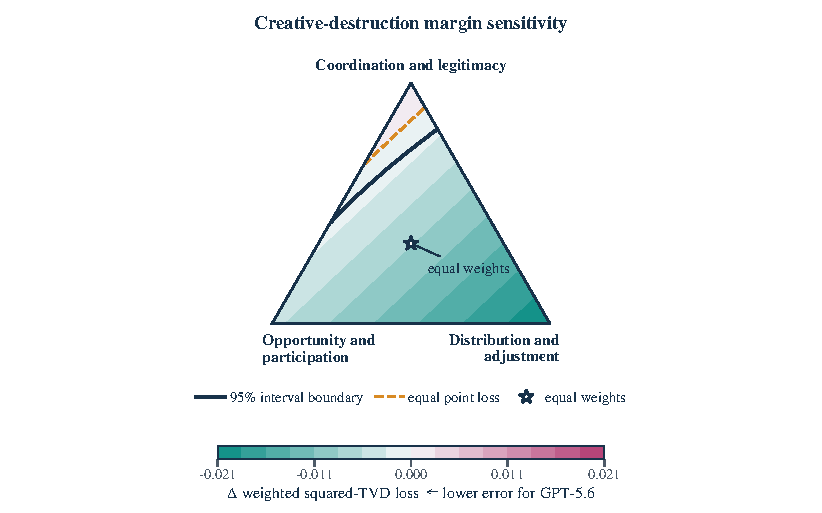
\includegraphics[width=\linewidth]{figs/figS3_economic_sensitivity.pdf}
\caption{Continuous sensitivity over nonnegative weights on opportunity, adjustment,
and coordination. Color encodes the GPT-5.6-minus-GPT-5.5 weighted squared-TVD loss;
teal is lower for GPT-5.6. The dashed amber contour marks equal point loss, the solid
navy contour the boundary where the 95\% interval first excludes zero, and the star equal
weights. This declared index is not observed welfare or a realized policy effect.}
\label{fig:economic-surface}
\end{figure}

\subsection{Transparent counterfactual bridge}
Let $h\in[0,1]^6$ be a society's observed value profile and let
$p=(i,a,s)'$ describe generic intensities of innovation support, adjustment assistance,
and safeguards. For an explicit local mapping $p^\star(h)=Bh$ and quadratic loss
\[
W(h,p)=\bar W-\frac12(p-Bh)'Q(p-Bh),\qquad Q\succ0,
\]
an adviser substituting $h+e$ for $h$ selects $B(h+e)$ and creates
\[
\mathcal R(e)=\frac12e'B'QBe\geq0.
\]
The result follows because $B'QB$ is positive semidefinite; regret is zero exactly when
$Be=0$. This establishes a mechanism: representation errors matter when they load onto
decision-relevant directions. The empirical margin index describes those directions in
the observed survey space; the quadratic bridge then shows their potential consequence
under an explicit local mapping.

\subsection{Implications for social adjustment}
A scalar model leaderboard cannot reveal whether an update changes the balance between
innovation incentives and transition burdens. Distributional fidelity, directional
bias, and cross-country geometry provide complementary diagnostics: the first captures
agreement on each issue, the second reveals which way the expected answer moves, and the
third tests whether differences among societies are preserved. This is the economic
reason EthosGPT treats model evolution as a vector of changes rather than a single
quality increment.
\FloatBarrier
